\lab{Iterative Solvers}{Iterative Solvers}
\label{lab:iter_methods}

\objective{
Many real-world problems of the form $A\x =\b$ have tens of thousands of parameters.
Solving such systems with Gaussian elimination or matrix factorizations could require trillions of floating point operations (FLOPs), which is of course infeasible.
Solutions of large systems must therefore be approximated iteratively.
In this lab, we implement three popular iterative methods for solving large systems: Jacobi, Gauss-Seidel, and Successive Over-Relaxation.}

% Though finding an exact solution is either very time intensive or unstable, iterative methods give a sufficiently close approximations and take much less time.

% TODO talk about LU-decomposition a bit and why we don't want to use it in this case.

\section*{Iterative Methods} % ================================================

The general idea behind any iterative method is to make an initial guess at the solution to a problem, apply a few easy computations to better approximate the solution, use that approximation as the new initial guess, and repeat until done.
Throughout this lab, we use the notation $\x^{(k)}$ to denote the $k$th approximation for the solution vector $\x$ and $x^{(k)}_i$ to denote the $i^{th}$ component of $\x^{(k)}$.
With this notation, every iterative method can be summarized as
\begin{equation}\x^{(k+1)} = f(\x^{(k)}),\label{eq:iter-summary}\end{equation}
where $f$ is some function used to approximate the true solution $\x$.

In the best case, the iteration converges to the true solution ($\x^{(k)}\rightarrow\x$).
In the worst case, the iteration continues forever without approaching the solution.
Iterative methods therefore require carefully chosen \emph{stopping criteria} to prevent iterating forever.
The general approach is to continue until the difference between two consecutive approximations is sufficiently small, and to iterate no more than a specific number of times.
More precisely, choose a very small $\epsilon > 0$ and an integer $N\in\mathbb{N}$, and update the approximation using Equation \ref{eq:iter-summary} until either
\begin{equation} % Stopping Criteria.
\|\x^{(k-1)}-\x^{(k)}\| < \epsilon
\qquad \text{or} \qquad
k > N.
\label{stopping-criteria}
\end{equation}

The choices for $\epsilon$ and $N$ are significant: a ``large'' $\epsilon$ (such as $10^{-6}$) produces a less accurate result than a ``small'' $\epsilon$ (such $10^{-16}$), but demands less computations; a small $N$ (10) also potentially lowers accuracy, but detects and halts non-convergent iterations sooner than with a large $N$ (10,000).

\section*{The Jacobi Method} % ================================================

The \emph{Jacobi Method} is a simple but powerful method used for solving certain kinds of large linear systems.
The main idea is simple: solve for each variable in terms of the others, then use the previous values to update each approximation.
As a (very small) example, consider the following $3 \times 3$ system.
\begin{align*}
\begin{array}{ccccccc}
  2x_1 &   &      & - & x_3  & = & 3  \\
  -x_1 & + & 3x_2 & + & 2x_3 & = & 3  \\
       & + & x_2  & + & 3x_3 & = & -1 \\
\end{array}
\end{align*}

Solving the first equation for $x_1$, the second for $x_2$, and the third for $x_3$ yields the following.
\begin{align*}
\begin{array}{ccc}
    x_1 & = & \frac{1}{2}(3 + x_3) \\
    x_2 & = & \frac{1}{3}(3 + x_1 - 2x_3) \\
    x_3 & = & \frac{1}{3}(-1 - x_2)
\end{array}
\end{align*}

Now begin with an initial guess $\x^{(0)} = [x^{(0)}_1, x^{(0)}_2, x^{(0)}_3]\trp = [0,0,0]\trp$.
To compute the first approximation $\x^{(1)}$, use the entries of $\x^{(0)}$ as the variables on the right side of the previous equation.
\begin{align*}
\begin{array}{ccccccc}
    x^{(1)}_1 & = & \frac{1}{2}(3 + x^{(0)}_3) & = & \frac{1}{2} (3 + 0) & = & \frac{3}{2} \\
    x^{(1)}_2 & = & \frac{1}{3}(3 + x^{(0)}_1 - 2x^{(0)}_3) & = & \frac{1}{3} (3 + 0 - 0) & = & 1 \\
    x^{(1)}_3 & = & \frac{1}{3}(-1 - x^{(0)}_2) & = & \frac{1}{3} (-1 - 0) & = & -\frac{1}{3} \\
\end{array}
\end{align*}

So $\mathbf{x}^{(1)} = [\frac{3}{2}, 1, -\frac{1}{3}]\trp$.
Computing $\mathbf{x}^{(2)}$ is similar.
\begin{align*}
\begin{array}{ccccccc}
x^{(2)}_1 & = & \frac{1}{2} ( 3 + x^{(1)}_3)  & = & \frac{1}{2} (3 - \frac{1}{3})     & = & \frac{4}{3} \\
x^{(2)}_2 & = & \frac{1}{3} ( 3 + x^{(1)}_1 - 2x^{(1)}_3) & = & \frac{1}{3} (3 + \frac{3}{2} + \frac{2}{3}) & = &  \frac{31}{18} \\
x^{(2)}_3 & = & \frac{1}{3} ( -1 - x^{(1)}_2)       & = & \frac{1}{3} (-1 - 1)    & = & -\frac{2}{3} \\
\end{array}
\end{align*}

The process is repeated until at least one of the two stopping criteria in Equation \ref{stopping-criteria} is met.
For this particular problem, convergence to 8 decimal places ($\epsilon = 10^{-8}$) is reached in 29 iterations.

\begin{center}
\begin{tabular}{c|ccc}
    & $x^{(k)}_1$ & $x^{(k)}_2$ & $x^{(k)}_3$ \\
    \hline
    $\x^{(0)}$ & 0 & 0 & 0 \\
    %\hline
    $\x^{(1)}$ & 1.5 & 1 & -0.33333 \\
    %\hline
    $\x^{(2)}$  & 1.33333333 & 1.72222222 & -0.66666667 \\
    $\x^{(3)}$  & 1.16666667 & 1.88888889 & -0.90740741 \\
    $\x^{(4)}$  & 1.04629630 & 1.99382716 & -0.96296296 \\
    \vdots      & \vdots     & \vdots     & \vdots      \\
    $\x^{(28)}$ & 0.99999999 & 2.00000001 & -0.99999999 \\
    $\x^{(29)}$ & 1          & 2          & -1          \\
\end{tabular}
\end{center}

\subsection*{Matrix Representation} % -----------------------------------------

The iterative steps performed above can be expressed in matrix form.
First, decompose $A$ into its diagonal entries, its entries below the diagonal, and its entries above the diagonal, as $A = D + L + U$.
\begin{align*}
\begin{array}{ccccc}
    \left[\begin{array}{cccc}
        a_{11} & 0 & \ldots & 0 \\
        0 & a_{22} & \ldots & 0 \\
        \vdots & \vdots & \ddots & \vdots \\
        0 & 0 & \ldots & a_{nn} \\
    \end{array}\right]
    & &
    \left[\begin{array}{cccc}
    0 & 0 & \ldots & 0 \\
    a_{21} &  0 & \ldots & 0\\
     \vdots & \ddots & \ddots & \vdots \\
    a_{n1} & \ldots & a_{n,n-1} & 0 \\
    \end{array}\right]
    & &
    \left[\begin{array}{cccc}
    0 & a_{12} & \ldots & a_{1n} \\
    0 & 0 & \ddots & \vdots \\
     \vdots & \vdots & \ddots & a_{n-1,n} \\
    0 & 0 & \ldots & 0 \\
    \end{array}\right]
    \\D & & L & & U
\end{array}
\end{align*}

With this decomposition, we solve for $\x$ in the following way.
\begin{align*}
A\x &= \b\\
(D + L + U)\x &= \b\\
D\x &= -(L+U)\x + \b\\
\x &= D^{-1}(-(L+U)\x + \b)
\end{align*}

Now using $\x^{(k)}$ as the variables on the right side of the equation to produce $\x^{(k+1)}$ on the left, and noting that $L+U=A-D$, we have the following.
\begin{align}
\nonumber \x^{(k+1)} &= D^{-1}(-(A-D)\x^{(k)} + \b) \\
\nonumber &= D^{-1}(D\x^{(k)} - A\x^{(k)}  + \b)\\
&= \x^{(k)} + D^{-1}(\b - A\x^{(k)})
\label{eq:jacobi-method}
\end{align}

There is a potential problem with Equation \ref{eq:jacobi-method}: calculating a matrix inverse is the cardinal sin of numerical linear algebra, yet the equation contains $D^{-1}$.
However, since $D$ is a diagonal matrix, $D^{-1}$ is also diagonal, and is easy to compute.
\[
D^{-1} =
\left[\begin{array}{cccc}
    \frac{1}{a_{11}} & 0                & \ldots & 0      \\
    0                & \frac{1}{a_{22}} & \ldots & 0      \\
    \vdots           & \vdots           & \ddots & \vdots \\
    0                & 0                & \ldots & \frac{1}{a_{nn}}
\end{array}\right]
\]

Because of this, the Jacobi method requires that $A$ have nonzero diagonal entries.

The diagonal $D$ can be represented by the 1-dimensional array $\mathbf{d}$ of the diagonal entries. %(instead of as a 2-dimensional array).
Then the matrix multiplication $D\x$ is equivalent to the component-wise vector multiplication $\mathbf{d}*\x = \x*\mathbf{d}$.
Likewise, the matrix multiplication $D^{-1}\x$ is equivalent to the component-wise ``vector division'' $\x/\mathbf{d}$.

% TODO: this isn't super useful, but we do need to demonstrate "vector division".
\begin{lstlisting}
>>> import numpy as np

>>> D = np.array([[2,0],[0,16]])    # Let D be a diagonal matrix.
>>> d = np.diag(D)                  # Extract the diagonal as a 1-D array.
>>> x = np.random.random(2)
>>> np.allclose(D.dot(x), d*x)
True
\end{lstlisting}

\begin{comment} % Jacobi algorithm box. Probably unnecessary.
\begin{algorithm}[H]
\begin{algorithmic}[1]
\Procedure{Jacobi Method}{$A$, $\b$, $\epsilon$, $N$}
    \State $m, n \gets \shape{A}$
        \Comment{Store the dimensions of $A$.}
    \State $\mathbf{d} \gets$ diag($A$)
        \Comment{Get the diagonal entries of $A$ with \li{np.diag()}.}
    \State $\x^{(0)} \gets \zeros{n}$
        \Comment{An array of $n$ zeros.}
    \For{$k=0 \ldots N-1$}
        \State $\x^{(k+1)} \gets (\b - A\x^{(k)} + \mathbf{d}*\x^{(k)})/\mathbf{d}$
        \If{$\|\mathbf{x}^{(k-1)} - \mathbf{x}^{(k)}\|_{\infty} < \epsilon$}
            \State \pseudoli{break}
        \EndIf
    \EndFor
    \State \pseudoli{return} $\x^{(k)}$
\EndProcedure
\end{algorithmic}
\caption{}
\label{alg:jacobi-method}
\end{algorithm}
\end{comment}

\begin{problem} % Implement the Jacobi Method.
Write a function that accepts a matrix $A$, a vector $\b$, a convergence tolerance $\epsilon$, and a maximum number of iterations $N$.
Implement the Jacobi method using Equation \ref{eq:jacobi-method}, returning the approximate solution to the equation $A\x = \b$.

Run the iteration until $\|\mathbf{x}^{(k-1)} - \mathbf{x}^{(k)}\|_{\infty} < \epsilon$, and only iterate at most $N$ times.
Avoid using \li{la.inv()} to calculate $D^{-1}$, but use \li{la.norm()} to calculate the vector $\infty$-norm $\|\x\|_\infty = \sup{|x_i|}$.

% \footnote{See Chapter 3 of Volume I for a technical definition of this norm.}

\begin{lstlisting}
>>> from scipy import linalg as la

>>> x = np.random.random(10)
>>> la.norm(x, <<ord>>=np.inf)          # Use la.norm() for ||x||.
0.74623726404168045
>>> np.<<max>>(np.<<abs>>(x))               # Use pure NumPy for ||x||.
0.74623726404168045
\end{lstlisting}

% TODO: Move this elsewhere...
% \begin{warn}
% NumPy arrays are mutable.
% Therefore, at each iteration, the values of $\x^{(k-1)}$ and $\x^{(k)}$ will need to be stored in two distinct copies.
% \end{warn}

Your function should be robust enough to accept systems of any size.
To test your function, use the following function to generate an $n\times n$ matrix $A$ for which the Jacobi method is guaranteed to converge.
Generate a random $\b$ with \li{np.random.random()}.

\begin{lstlisting}
def diag_dom(n, num_entries=None):
    """Generate a strictly diagonally dominant nxn matrix.

    Inputs:
        n (int): the dimension of the system.
        num_entries (int): the number of nonzero values
            Defaults to n^(3/2)-n.

    Returns:
        A ((n,n) ndarray): An nxn strictly diagonally dominant matrix.
    """
    if num_entries is None:
        num_entries = int(n**1.5) - n
    A = np.zeros((n,n))
    rows = np.random.choice(np.arange(0,n), size=num_entries)
    cols = np.random.choice(np.arange(0,n), size=num_entries)
    data = np.random.randint(-4, 4, size=num_entries)
    for i in xrange(num_entries):
        A[rows[i], cols[i]] = data[i]
    for i in xrange(n):
        A[i,i] = np.<<sum>>(np.<<abs>>(A[i])) + 1
    return A
\end{lstlisting}

Also test your function on random $n \times n$ matrices
If the iteration is non-convergent, the successive approximations will have increasingly large entries.

\label{prob:jacobi}
\end{problem}

\subsection*{Convergence} % ---------------------------------------------------

Most iterative methods only converge under certain conditions.
For the Jacobi method, convergence mostly depends on the nature of the matrix $A$.
If the entries $a_{ij}$ of $A$ satisfy the property \[|a_{ii}| > \sum_{j \neq i} |a_{ij}|\ \text{for all}\ i = 1,2,\hdots,n,\] then $A$ is called \emph{strictly diagonally dominant} (for example, \li{diag_dom()} in Problem \ref{prob:jacobi} generates a strictly diagonally dominant $n\times n$ matrix).
If this is the case, then the Jacobi method always converges, regardless of the initial guess $\x_0$.%
\footnote{Although this seems like a strong requirement, most real-world linear systems can be represented by strictly diagonally dominant matrices.
}
Other iterative methods, such as Newton's method, depend mostly on the initial guess.

There are a few ways to determine whether or not an iterative method is converging.
For example, since the approximation $\x^{(k)}$ should satisfy $A\x^{(k)} \approx \b$, the normed difference $\|A\x^{(k)} - \b\|_\infty$ should be small.
This value is called the \emph{absolute error} of the approximation.
If the iterative method converges, the absolute error should decrease to $\epsilon$.

\begin{problem}
Modify your Jacobi method function in the following ways:
\begin{enumerate}
    \item Add a keyword argument called \li{plot}, defaulting to \li{False}.
    \item Keep track of the absolute error $\|A\mathbf{x}^{(k)} - \mathbf{b}\|_{\infty}$ of the approximation for each value of $k$.
    \item If \li{plot} is \li{True}, produce a lin-log plot the error against iteration count (use \li{plt.semilogy()} instead of \li{plt.plot()}).
    Return the approximate solution $\x$ even if \li{plot} is \li{True}.
\end{enumerate}
If the iteration converges, your plot should resemble the following figure.

\begin{figure}[H]
    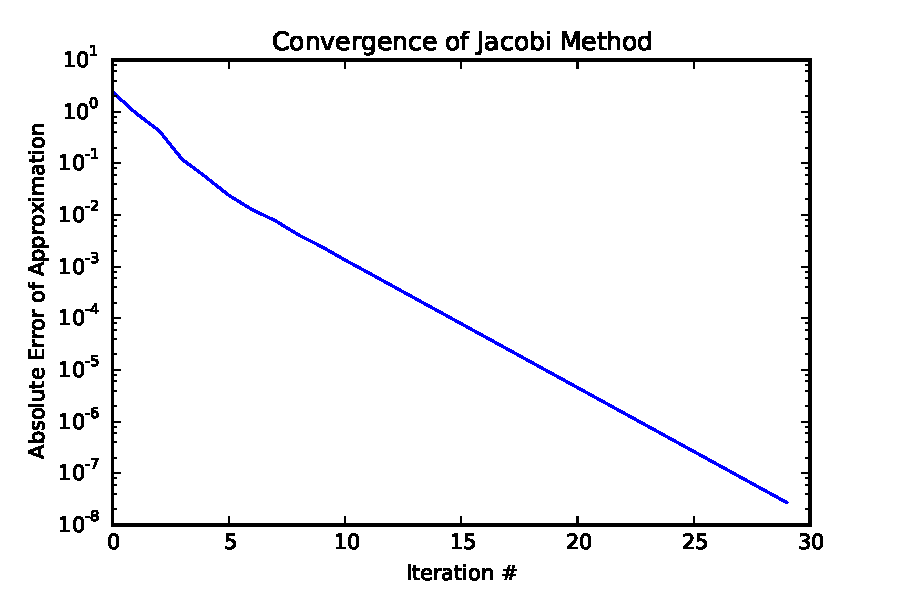
\includegraphics[width=.7\textwidth]{jacobi_convergence.pdf}
\end{figure}
\end{problem}

\section*{The Gauss-Seidel Method} % ==========================================

The Gauss-Seidel method is quite similar to the Jacobi method. We will examine
the same system as before. The main difference between Gauss-Seidel and Jacobi
is that in Gauss-Seidel, any new information is used immediately. As with Jacobi,

$$
\begin{matrix}
x^{(1)}_1 & = & \frac{1}{2} ( 3 + x^{(0)}_3)  & = & \frac{1}{2} (3 + 0)     & = & \frac{3}{2} \\
\end{matrix}
$$

But now, we use this updated value of $x^{(1)}_1$ in our calculation of
$x^{(1)}_2$ as follows
$$
\begin{matrix}
x^{(1)}_2 & = & \frac{1}{3} ( 3 + x^{(1)}_1 - 2x^{(0)}_3) & = & \frac{1}{3} (3 + \frac{3}{2} - 0) & = & \frac{3}{2} \\
\end{matrix}
$$

We now can use the updated values of $x^{(1)}_1$ and $x^{(1)}_2$ in our
calculation of $x^{(1)}_3$,
$$
\begin{matrix}
x^{(1)}_3 & = & \frac{1}{3} ( -1 - x^{(1)}_2)       & = & \frac{1}{3} (-1 - \frac{3}{2})    & = & -\frac{5}{6}
\end{matrix}.
$$

This process of using what we have calculated immediately is called
\emph{forward substitution}. Using forward substitution causes the algorithm to
converge much faster.

\begin{center}
    \begin{tabular} {c | c c c}
        & $x^{(k)}_1$ & $x^{(k)}_2$ & $x^{(k)}_3$ \\
        \hline
          $x^{(0)}$ & 0 & 0 & 0 \\
          %\hline
          $x^{(1)}$ & 1.5 & 1.5 & -0.833333 \\
          %\hline
          $x^{(2)}$ & 1.08333333 & 1.91666667 & -0.97222222 \\
          $x^{(3)}$ & 1.01388889 & 1.98611111 & -0.99537037 \\
          $x^{(4)}$ & 1.00231481 & 1.99768519 & -0.9992284 \\
          \vdots    & \vdots    & \vdots     & \vdots     \\
          $x^{(11)}$ & 1.00000001 & 1.99999999 & -1 \\
          $x^{(12)}$ & 1 & 2 & -1 \\
        \end{tabular}
\end{center}
Notice that Gauss-Seidel converged in less than half as many iterations.

As shown above, Gauss-Seidel updates one element of the solution vector at a time.
This process is more generally described by the following equation.

\begin{equation} \label{eq:gauss_seidel_full}
x^{(k+1)}_i = \frac{1}{a_{ii}} \left (b_i - \sum_{j < i}a_{ij}x^{(k+1)}_j - \sum_{j > i}a_{ij}x^{(k)}_j \right )
\end{equation}

Notice that the two sums closely resemble an inner product without the
$i^{\text{th}}$ term. If we update the entries of the vector $\mathbf{x}$ in place,
this equation can be represented as,

$$
x^{(k+1)}_i = \frac{1}{a_{ii}} \left ( b_i - \left < A_i, \mathbf{x}^{(k)} \right > + a_{ii}x^{(k)}_i \right )
$$
where $A_i$ is the $i^{th}$ row of $A$. This can be simplified further to

\begin{equation} \label{eq:gauss_seidel}
x^{(k+1)}_i = x^{(k)}_i + \frac{1}{a_{ii}} \left ( b_i - \left < A_i, \mathbf{x}^{(k)}\right >\right)
\end{equation}

Making one sweep through all the entries of $x$ completes one iteration. We
continue this same process until convergence is attained.

\begin{problem} \label{prob:gauss_seidel}
Implement the Gauss-Seidel method using Equation \ref{eq:gauss_seidel}. Your
function should accept a matrix \li{A}, a vector \li{b}, an optional parameter
\li{tol} that defaults to \li{1e-8} and an optional parameter \li{maxiters} that
defaults to $100$. Your function should return the solution vector \li{x} as
well as a list of all the approximations of \li{x} at each iteration. HINT: It is
easiest to implement this algorithm if you update the approximation vector, $x^{(k)}$, in-place.
\end{problem}

\subsection*{Convergence of Gauss-Seidel} % -----------------------------------

\begin{definition}
    A matrix $A \in M_n(\mathbb{R})$ is \emph{positive definite} if all its
    eigenvalues are positive.
\end{definition}

\begin{theorem}
    The Gauss-Seidel method converges for a matrix $A$ if it is strictly
    diagonally dominant or positive definite.
\end{theorem}

For a treatment on the theory of positive definite matrices, see Chapter ?? of
Volume 1 of the textbook.

\begin{problem}
As we have described up to this point in the lab, we can take advantage of the
sparsity of a linear system by using iterative methods like Jacobi and Gauss-Seidel.
For this problem, compare the runtimes between your \li{gauss_seidel()} function and
\li{la.solve()} for a strictly diagonally dominant system of 5000 parameters. Use the following
code to generate a strictly diagonal dominant matrix:
\begin{lstlisting}
def diag_dom(n, num_entries=None):
    """Generate a strictly diagonally dominant nxn matrix.

    Inputs:
        n (int) - dimension.
        vals (list) - range of values for off-diagonal entries.
        num_entries (int) - number of nonzero values. If None, num_entries
                    defaults to n^(1.5) - n.

    Returns:
        A (array) - nxn strictly diagonally dominant matrix.
    """
    if num_entries is None:
        num_entries = int(n**1.5) - n
    A = np.zeros((n,n))
    i = np.random.choice(np.arange(0,n), size=num_entries)
    j = np.random.choice(np.arange(0,n), size=num_entries)
    data = np.random.randint(-4,4,size=num_entries)
    for c in xrange(num_entries):
        A[ i[c], j[c] ] = data[c]
    for i in xrange(n):
        A[i,i] = np.sum(np.abs(A[i,:])) + 1
    return A
\end{lstlisting}
What difference do you see between these two functions? Explain why there is such a big difference.
\end{problem}

\section*{Sparse Systems} % ===================================================

Some linear systems may have tens of thousands of parameters.
However, in applications where systems of this size arise, it is also common
that such matrices are sparse.
The tools in SciPy's \li{sparse} library make it possible to work with even these very large systems.

\begin{comment}
The following is a quick example of how the different types of sparse matrices
can be used to optimize performance.

\begin{lstlisting}
# Initialize the matrix using a coo_matrix.
>>> rows = np.array([0,1,2,3,0,2])
>>> cols = np.array([0,1,2,3,1,0])
>>> values = np.array([3,5,4,1,2,1])
>>> A = spar.coo_matrix((values, (rows,cols)), shape=(4,4))

# To visualize the matrix, use .todense(). Keep in mind doing
#   operations on this dense matrix forfeits all sparse-related
#   optimizations.
>>> print A.todense()
matrix([[3, 2, 0, 0],
        [0, 5, 0, 0],
        [1, 0, 4, 0],
        [0, 0, 0, 1]])

# perform matrix multiplicaton after converting to a csr_matrix.
>>> Acsr = A.tocsr()
>>> x = np.array([1,0,-1,2])
>>> b = Acsr.dot(x)
array([3,0,-3,2])

# access rows of a csr_matrix. The syntax for slicing a csr_matrix
#  (and csc_matrix) is identical to slicing NumPy arrays. For row slicing,
#  use a csr_matrix. For column slicing, use a csc_matrix.
>>> Acsr[0,:].todense()
matrix([[3, 2, 0, 0]])

>>> Acsc = A.tocsc()
>>> Acsc[:,2].todense()
matrix([[0],
        [0],
        [4],
        [0]])

# access individual elements of the matrix after converting to a dok_matrix.
>>> Adok = A.todok()
>>> print Adok[2,0]
1
>>> print Adok[1,1]
5
\end{lstlisting}

Since the \li{coo_matrix} type allows for fast sparse matrix type conversion, it is usually worth the time and memory to convert to the sparse matrix type that corresponds with the operations you are performing.
\end{comment}


\begin{problem} % Gauss-Seidel with Sparse matrices.
To be able to use the Gauss-Seidel method on sparse matrices, you must translate
the code you wrote in Problem \ref{prob:gauss_seidel} from \li{numpy} to \li{scipy.sparse}.
The algorithm is the same, but there are some functions that are named differently
between these two packages.

Write a new function that accepts a sparse matrix \li{A}, a NumPy array \li{b},
an optional parameter \li{tol} that defauls to \li{1e-8}, and an optional parameter
\li{maxiters} that defaults to 100. Your function should return the solution
vector \li{x} as well as a list of all the approximations of \li{x} at each
iteration.

We want this function to run as quickly as possible. The Gauss-Seidel method calls for us to extract rows from the matrix $A$ then multiply by the vector $x$. There are many ways to do this that cause some fairly serious runtime issues, so we will provide the code for this specific portion of the algorithm.

\begin{lstlisting}
# Slice the i-th row of A and dot product the vector x
rowstart = A.indptr[i]
rowend = A.indptr[i+1]
Aix = np.dot(A.data[rowstart:rowend], x[A.indices[rowstart:rowend]])
\end{lstlisting}

To test your function, you can create a strictly diagonally dominant matrix with
the following code. In this code, also note how different types of sparse matrices
have been used to optimize performance.

\begin{lstlisting}
def spar_diag_dom(n, num_entries=None):
    """Generate a strictly diagonally dominant sparse nxn matrix.

    Inputs:
        n (int) - dimension
        num_entries (int) - number of nonzero values. If None, num_entries
                    defaults to n^(1.5) - n.

    Returns:
        A (spar.csr_matrix) - strictly diagonally dominant sparse nxn matrix.
    """
    return spar.csr_matrix(diag_dom(n, num_entries=num_entries))
\end{lstlisting}

\end{problem}

\subsection*{Successive Over-Relaxation (SOR)} % ------------------------------------

There are some systems that meet the requirements for convergence in the
Gauss-Seidel method that do not converge very quickly. A slightly altered version
of the Gauss-Seidel method has been developed that can result in faster convergence.
This is achieved by introducting a relaxation factor, $\omega$. This method is
called Successive Over-Relaxation. In fact, for many slowly converging iterative processes, convergence can be improved by introducing a relaxation factor.

The iterative equation for Gauss-Seidel, Equation \ref{eq:gauss_seidel_full},
with the introduction of a relaxing factor $\omega$ becomes,

$$
x_i^{(k+1)} = (1 - \omega)x_i^{(k)} + \frac{\omega}{a_{ii}} \left (b_i - \sum_{j < i}a_{ij}x^{(k+1)}_j - \sum_{j > i}a_{ij}x^{(k)}_j \right )
$$

Updating the solution vector $x$ inplace as we did with Gauss-Seidel, this
equation becomes,

\begin{equation} \label{eq:sor}
x^{(k+1)}_i = x^{(k)}_i + \frac{\omega}{a_{ii}} \left ( b_i - \left < A_i, \mathbf{x}^{(k)} \right > \right )
\end{equation}

Equation \ref{eq:sor} follows by simplifying the full analytic equation in the
same way we simplified the Gauss-Seidel method. Notice that when $\omega = 1$,
Successive Over-Relaxation is equivalent to Gauss-Seidel.

\begin{problem}
Implement Successive Over-Relaxation. You should be able to write
this function by changing one line of your code from your Gauss Seidel
function. Your function should be able to handle sparse matrices.

We will examine how varying the values of $\omega$ affects convergence in Problem \ref{prob:application}
\end{problem}

\section*{Application: Finite Difference Method} % ======================================================

Throughout this lab, we have said there are sparse linear systems that arise in applications that have tens of thousands of parameters. Systems of this size
often arise in Finite Difference problems. The underlying theory behind such problems will be addressed in Volume 4 of the textbook. We now present one such problem.


\begin{problem} \label{prob:application}

A common equation that occurs in both pure and applied mathematics is Laplace's equation.

\[ \frac{\partial^2 u}{\partial x^2}+ \frac{\partial^2 u}{\partial y^2}= 0.\]

We can use Laplace's Equation to model steady-state heat flow. Imagine we have a square metal plate where the top and bottom sides are fixed at 0 degrees Celcius and the left and right sides are fixed at 100 degrees Celcius. We can use Laplace's Equation to approximate the temperature of the interior of the metal plate at any given point.

For this problem we will solve Laplace's equation numerically using a technique called \textit{the finite difference method}.  The derivation of the finite difference method will be saved until the lab on Numerical Differentiation, but the relevant equations will be given here.

The finite difference method can be reduced to solving a sparse system of linear equations. We will describe how to initialize this linear system, but again, all the derivation will be saved for the lab on Numerical Differentiation.

In Figure \ref{fig:application} we have the basic set up of the problem described above. The metal plate being represented is $10 in \times 10 in$. The points $u_{i,j}$ are the discretized grid points we will use to approximate the temperature across the plate.

Then at an interior point of the grid, Laplace's equation can be approximated by
\begin{equation} \label{eq:laplace}
\begin{split}
    \frac{\partial^2 u_{i,j}}{\partial x^2}+ \frac{\partial^2 u_{i,y}}{\partial y^2} \approx \frac{1}{h^2}\left[-4u_{i,j} + u_{i+1,j} + u_{i-1,j} + u_{i,j+1} +  u_{i,j-1}\right]
\end{split}
\end{equation}
where $h$ is the distance between gridlines.

Writing Equation \ref{eq:laplace} for the $9$ interior points of the grid in Figure \ref{fig:application}result in a $9 \times 9$ system, $A \mathbf{x} = b$.

$$
\begin{bmatrix}
-4 & 1  &  0 &  1 &  0 &  0 &  0 &  0 & 0 \\
 1 & -4 &  1 &  0 &  1 &  0 &  0 &  0 & 0 \\
 0 & 1  & -4 &  0 &  0 &  1 &  0 &  0 & 0 \\
 1 & 0  &  0 & -4 &  1 &  0 &  1 &  0 & 0 \\
 0 & 1  &  0 &  1 & -4 &  1 &  0 &  1 & 0 \\
 0 & 0  &  1 &  0 &  1 & -4 &  0 &  0 & 0 \\
 0 & 0  &  0 &  1 &  0 &  0 & -4 &  1 & 0 \\
 0 & 0  &  0 &  0 &  1 &  0 &  1 & -4 & 1 \\
 0 & 0  &  0 &  0 &  0 &  1 &  0 &  1 & -4 \\
\end{bmatrix}
\begin{bmatrix}
u_{1,1} \\
u_{1,2} \\
u_{1,3} \\
u_{2,1} \\
u_{2,2} \\
u_{2,3} \\
u_{3,1} \\
u_{3,2} \\
u_{3,3} \\
\end{bmatrix}
=
\begin{bmatrix}
-100 \\
 0  \\
-100 \\
-100 \\
 0  \\
-100 \\
-100 \\
 0  \\
-100 \\
\end{bmatrix}
$$
For any positive integer n, the corresponding system $A \mathbf{x} = b$ can be expressed as,
$$
A = \begin{bmatrix}
B_1 & I &      &        & \\
I & B_2 &  I   &        & \\
  & I & \ddots & \ddots & \\
  &   & \ddots & \ddots & I \\
  &   &        &    I   & B_n
\end{bmatrix}
$$
where $B_i$, is an $n \times n$ matrix,
$$
B_i = \begin{bmatrix}
-4 &  1 &      &        & \\
 1 & -4 &  1   &        & \\
   &  1 & \ddots & \ddots & \\
   &    & \ddots & \ddots & 1 \\
   &    &        &    1   & -4
\end{bmatrix}.
$$
So the resulting matrix $A$ ends up being of size $n^2 \times n^2$.

For the vector $b$, all nonzero entries correspond to interior points that touch the left or right boundaries. The vector $b$ will be $n^2 \times 1$.

For this problem, do the following:
\begin{enumerate}
    \item Write a function \li{finite_difference()} that accepts an integer $n$ for the number of interior gridlines. Your function should return the corresponding sparse matrix $A$ and NumPy array $b$. For example, a value of $n = 3$ should result in the matrix $A$ and vector $b$ described above. HINT: Consider using \li{scipy.sparse.block_diag} and the \li{setdiag()} method of scipy sparse matrices for dynamically creating the matrix $A$.
    \item To demonstrate how convergence is affected by the value of $\omega$, time your \li{sparse_sor()} function for values of $\omega = [1, 1.05, 1.1, \dots , 1.9, 1.95 ]$. Plot your timings as a function of $\omega$. Generate the system $A \mathbf{x} = b$ using your \li{finite_difference()} function and a value of $n = 20$. Remember that $\omega = 1$ corresponds to the Gauss-Seidel method. How does Gauss-Seidel compare to SOR with the optimal $\omega$?

    NOTE: Notice that the matrix $A$ is not strictly diagonally dominant. However, this matrix is positive definite, so the algorithm will converge. Unfortunately, convergence for these kinds of systems require many more iterations. When using the \li{sparse_sor()} function in this problem, set \li{maxiters = 10000} and \li{tol=10**-2}.
    \item Using \li{plt.pcolormesh}, create a heatmap to visualize your solution. The solution vector you get from your \li{sparse_sor()} function will need to be reshaped to properly visualize the result.
\end{enumerate}

\begin{comment}
The following code generates a heatmap to help you visualize the steady-state heat flow across the interior of the plate:

\begin{lstlisting}
from matplotlib import pyplot as plt
import numpy as np

n = 50
A,b = finite_difference(n)
x = sparse_sor(A,b,1.9,maxiters=10000,tol=10**-2)[0]
U = x.reshape(n,n)
x,y = np.linspace(0,10,n), np.linspace(0,10,n)
X,Y = np.meshgrid(x,y)

plt.pcolormesh(X,Y,U,cmap='RdBu_r')
plt.show()
\end{lstlisting}
\end{comment}


\end{problem}

%\newpage

%\section*{Additional Material} % ==============================================



\begin{comment} % Migrated from NumPy lab. vvvvvvvvvvvvvvvvvvvvvvvvvvvvvvvvvvvv
\begin{algorithm} % Laplace's equation procedure.
\begin{algorithmic}[1]
\Procedure{Jacobi}{$n$, tol}
\State $U \gets$ an $n\times n$ array of zeros.
\State Set the boundaries of $U$.
\State $U^\prime \gets$ a copy of $U$.
\State diff $\gets$ tol
\While {diff $\ge$ tol}
    \State Set all interior points of $U^\prime$ equal to the average of their neighbors.
    \State diff $\gets$ the maximum of the absolute value of $U - U^\prime$.
    \State Interior of $U \gets$ interior of $U^\prime $.
\EndWhile
\State \pseudoli{return} $U$
\EndProcedure
\end{algorithmic}
\caption{The Jacobi method for solving Laplace's equation.}
\label{alg:jacobi}
\end{algorithm}

\begin{problem}
Laplace's equation is used to model steady-state heat flow on a square plate.
The plate can be approximated by a matrix, where each entry of the matrix represents the average temperature over a small square portion of the plate.
Suppose the plate starts at $0^\circ$ Celsius everywhere except on the east and west boundaries, which are held at a constant temperature of $100^\circ$.
In addition, the north and south boundaries are held constant at $0^\circ$.

\[
U = \left[\begin{array}{ccccc}
\textcolor[rgb]{0.,0.,1.}0 & \textcolor[rgb]{0.,0.,1.}0 & \textcolor[rgb]{0.,0.,1.}\cdots & \textcolor[rgb]{0.,0.,1.}0 & \textcolor[rgb]{0.,0.,1.}0\\
\textcolor[rgb]{1.,0.,0.}{100} & 0 & \cdots & 0 & \textcolor[rgb]{1.,0.,0.}{100}\\
\textcolor[rgb]{1.,0.,0.}\vdots & \vdots & \ddots & \vdots & \textcolor[rgb]{1.,0.,0.}\vdots \\
\textcolor[rgb]{1.,0.,0.}{100} & 0 & \cdots & 0 & \textcolor[rgb]{1.,0.,0.}{100}\\
\textcolor[rgb]{0.,0.,1.}0 & \textcolor[rgb]{0.,0.,1.}0 & \textcolor[rgb]{0.,0.,1.}\cdots & \textcolor[rgb]{0.,0.,1.}0 & \textcolor[rgb]{0.,0.,1.}0\\

\end{array}\right]
\]

The non-boundary, interior portion of the matrix (with black text) can be accessed with the slice \li{U[1:-1,1:-1]}.
To find the steady state of the hot plate, set each entry of the interior of $U$ equal to the average of its 4 immediate neighbors (the entries above, below, and to the left and right).
This step should take only \emph{one line} and should be based entirely on array slicing.

Continue updating the interior entries of $U$ until they stop changing significantly.
The entire procedure is summarized in Algorithm \ref{alg:jacobi}.

(Hint: The slice \li{U[:-2,1:-1]} references the upper neighbors of the interior points of $U$ and \li{U[1:-1,2:]} references the right neighbors. How can you reference the lower and left neighbors?)

Use the following code to visualize your results.
%% This does 3D visualization, but it's easier (and better) as a heat map.
% from mpl_toolkits.mplot3d import Axes 3D

%     x, y = np.linspace(0, 1, n), np.linspace(0, 1, n)
%     X, Y = np.meshgrid(x, y)
%     fig = plt.figure()
%     ax = fig.gca(projection='3d')
%     ax.plot_surface(X, Y, U, rstride=5)
%     plt.show()

\begin{lstlisting}
from matplotlib import pyplot as plt

def jacobi(n=100, tol=1e-8):

    # Perform the algorithm, storing the result in the array 'U'.

    # Visualize the results.
    plt.imshow(U)
    plt.show()
\end{lstlisting}

This Jacobi iteration is a \emph{finite difference method}, and is similar to many of the methods that we will use to find numerical solutions to differential equations in Volume IV.
\end{problem}

\begin{figure}[H]
\centering
\begin{subfigure}{.5\textwidth}
    \centering
    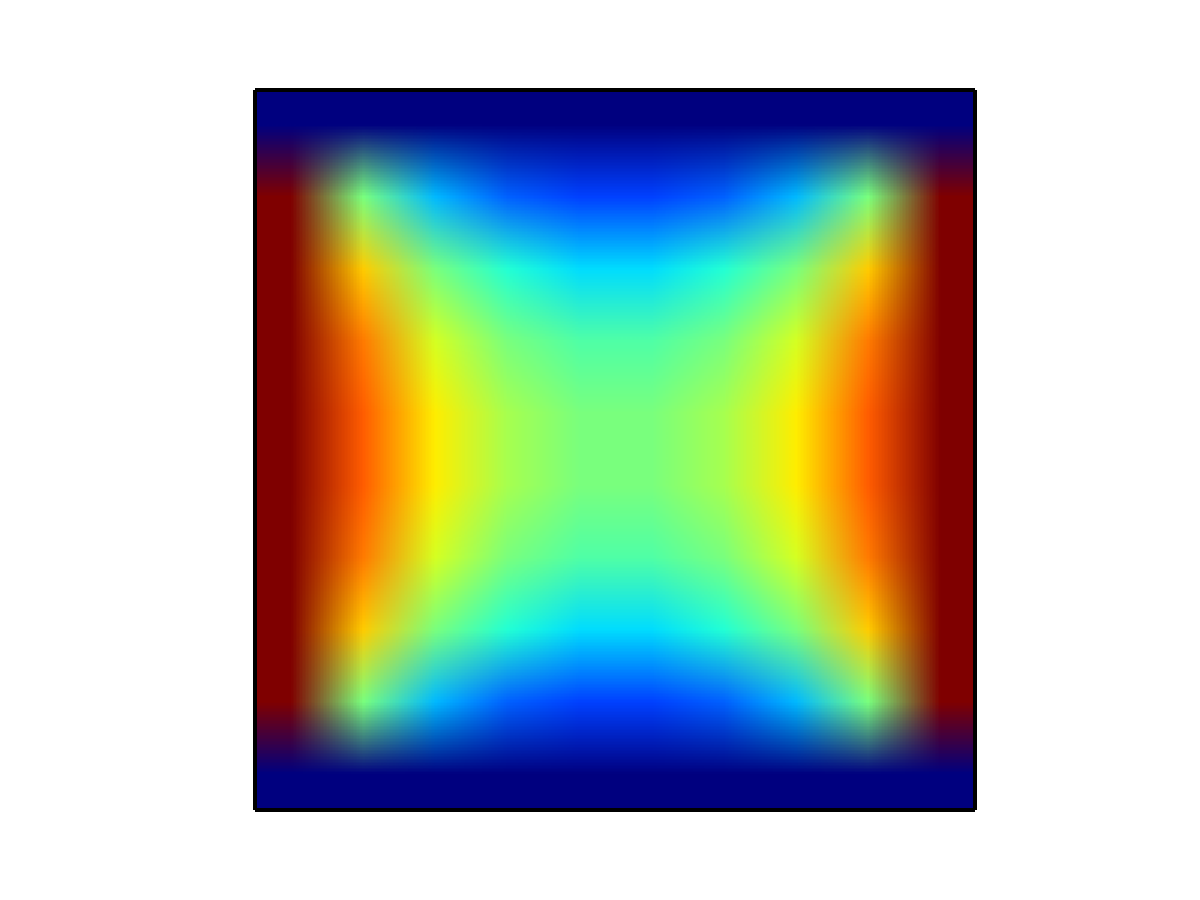
\includegraphics[width=\linewidth]{jacobi_small.pdf}
    \caption{$10\times 10$ approximation.}
\end{subfigure}%
\begin{subfigure}{.5\textwidth}
    \centering
    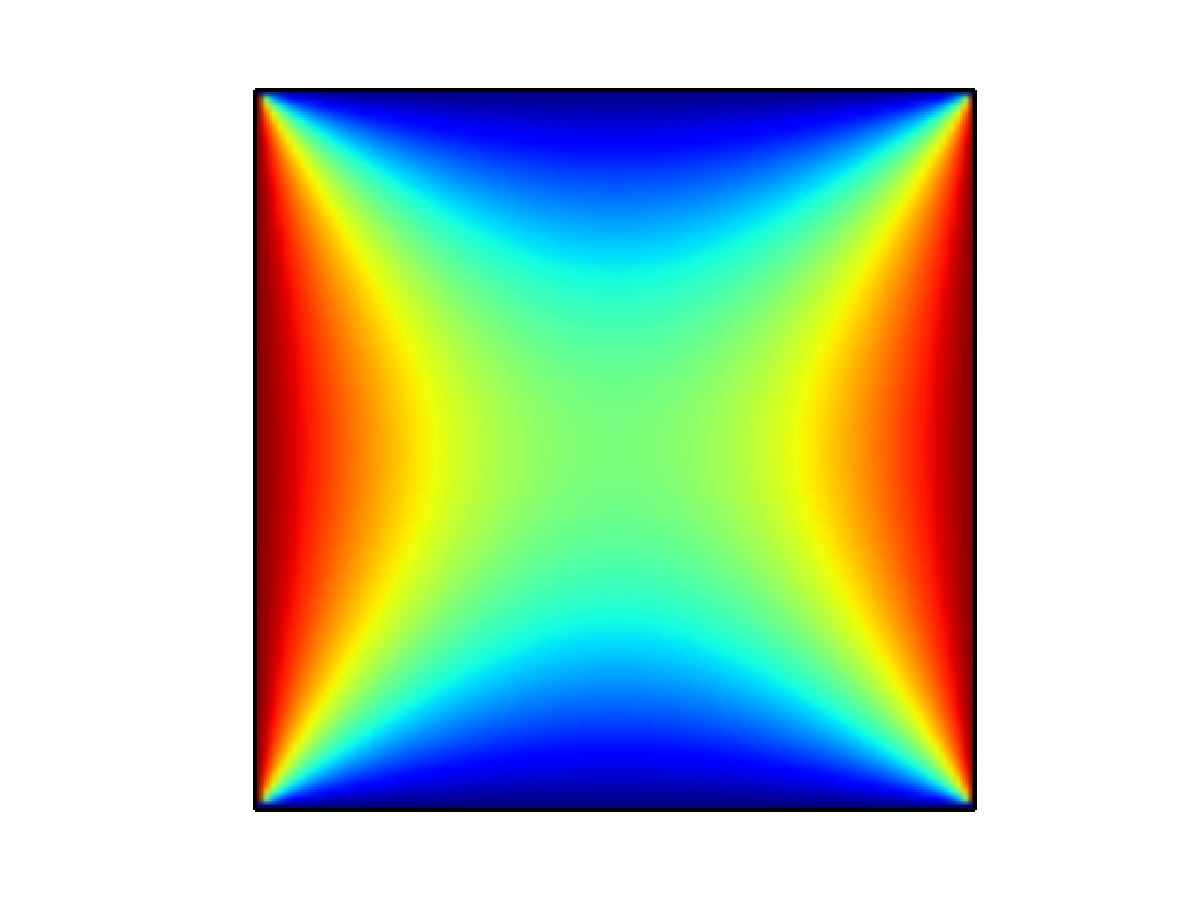
\includegraphics[width=\linewidth]{jacobi_big.pdf}
    \caption{$100\times 100$ approximation.}
\end{subfigure}
\caption{Hot plates in steady state with different resolutions.}
\end{figure}
\end{comment} % Used to be in NumPy ^^^^^^^^^^^^^^^^^^^^^^^^^^^^^^^^^^^^^^^^^^^
